\chapter{Implementación}

\section{Introducción}
\label{sec:intro}

Para la extracción de datos se ha utilizado, como se ha mencionado anteriormente, la herramientas Gephi.

\section{Estructura de la red}

En la red extraída los nodos son los protagonistas y las aristas son la interacción entre los mismos, por tanto se trata de una red dirigida.
\\ \\
La red original consta de 77 nodos y 254 aristas. Aunque le hemos intentado aplicar la componente gigante esta red no reduce su numero de aristas. Al ser tan pequeña la red no nos impide trabajar con ella de forma eficiente.
\\ \\

\section{Valores de medidas de análisis}
\label{sec:medidas}

\subsection{Red original}

\begin{figure}[H]
	\centering
	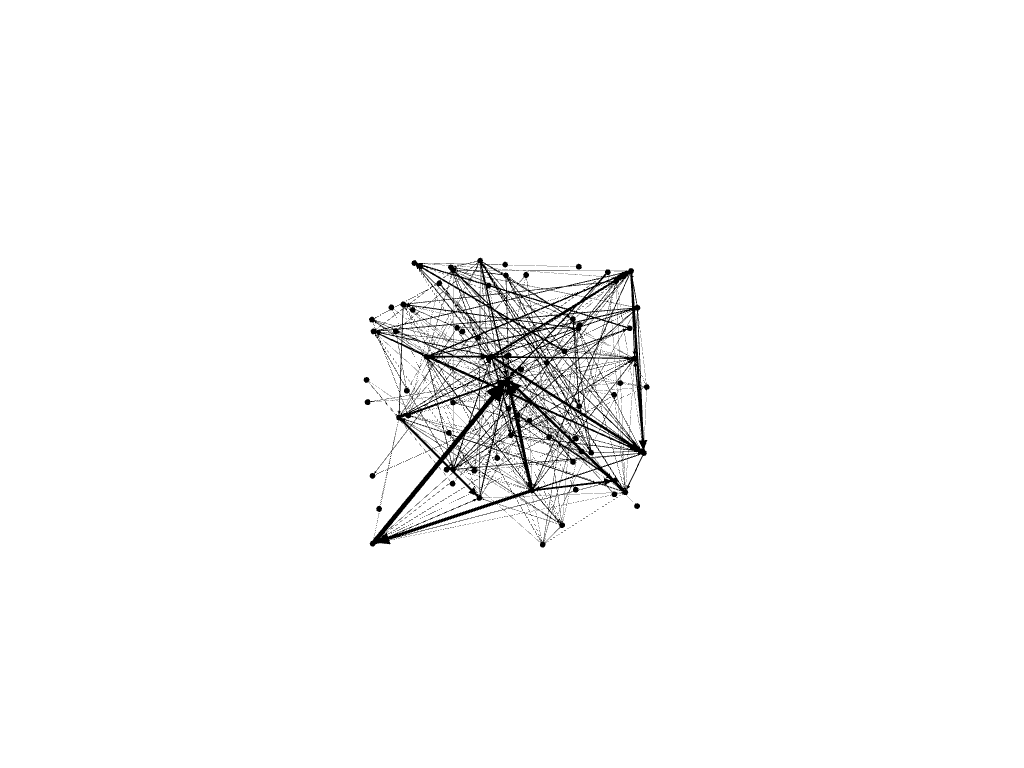
\includegraphics[width=12cm]{../images/original-graph}
	\caption{Grafo de la red original}
\end{figure}

\begin{table}[H]
	\centering
	\caption{Valores de las medidas de análisis de la red original}
	\label{tab:medidas-original}
	\begin{tabular}{| l | l |}
		\hline
		Medida                							& Valor          \\ 
		\hline
		Número de nodos ($N$)           					& 77           \\
		Número de enlaces ($L$)                   		& 254           \\
		Densidad ($D$)                   				& 0,043         \\
		Grado medio ($k$)                   				& 3,299          \\
		Diámetro ($d_{max}$)             				& 5              \\
		Distancia media ($d$)                   			& 2,4          \\
		Coeficiente clustering medio($C$)              	& 0,287          \\
		Componentes conexas   							& 1            \\ 
		\hline
	\end{tabular}
\end{table}

La densidad de la red original es muy pequeña.
\\ \\
La distancia media de un nodo a otro es muy pequeña lo cual es lógico al haber nodos que están conectados con un enorme número de usuarios. Además, el diámetro es de tan solo 5, por lo que, como muchos en 5 pasos, se podría pasar de un nodo a cualquier otro.
\\ \\

\section{Propiedades de la red}

A continuación se describirán propiedades de la red ya filtrada, que será sobre la que se haga la detección de comunidades y visualización.

\subsection{Distribución de grados}

\begin{figure}[H]
	\centering
	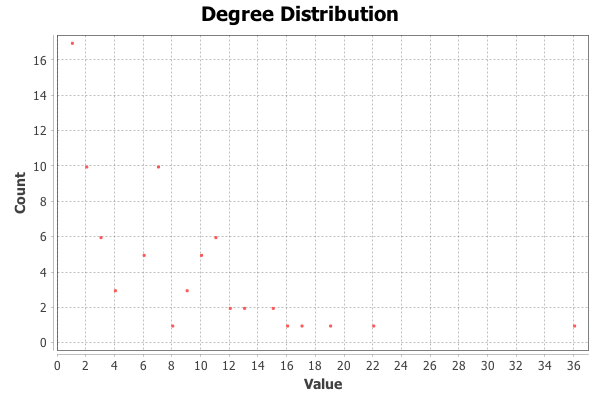
\includegraphics[width=12cm] {../images/degree-distribution}
	\caption{Distribución de grados para la red filtrada}
	\label{fig:degree-distribution}
\end{figure}

\begin{figure}[H]
	\centering
	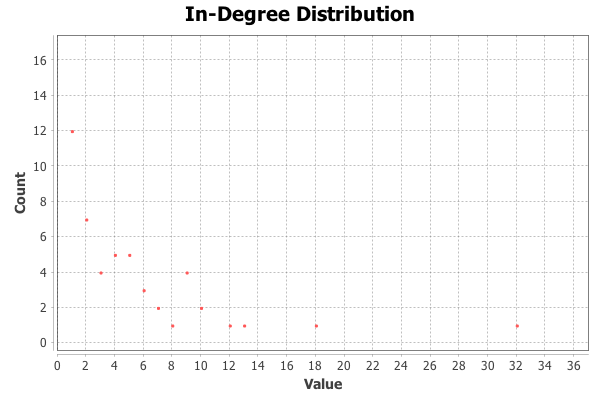
\includegraphics[width=12cm]{../images/in-degree-distribution}
	\caption{Distribución de grados de entrada para la red filtrada}
	\label{fig:in-degree-distribution}
\end{figure}

\begin{figure}[H]
	\centering
	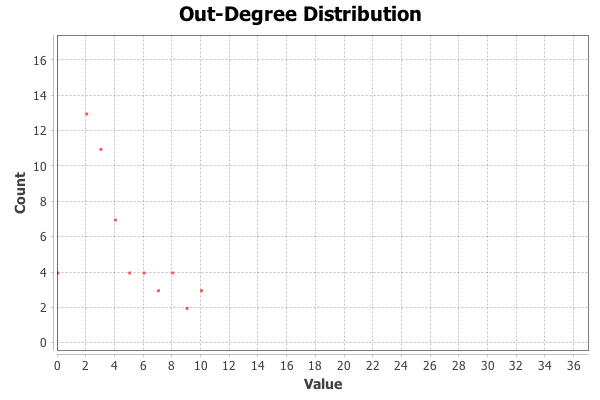
\includegraphics[width=12cm]{../images/out-degree-distribution}
	\caption{Distribución de grados de salida para la red filtrada}
	\label{fig:out-degree-distribution}
\end{figure}

Se puede observar como se cumple la ley de la potencia: $ P(k) \sim k^{-\gamma} $ y es que la mayoría de los nodos tienen pocos enlaces pero hay unos cuantos \textit{hubs} que tienen muchos, y posteriormente, al visualizarlo se verá una forma de estrella alrededor de estos. Por tanto podríamos decir que la red es libre de escala.

\subsection{Distribución de distancias}

\begin{figure}[H]
	\centering
	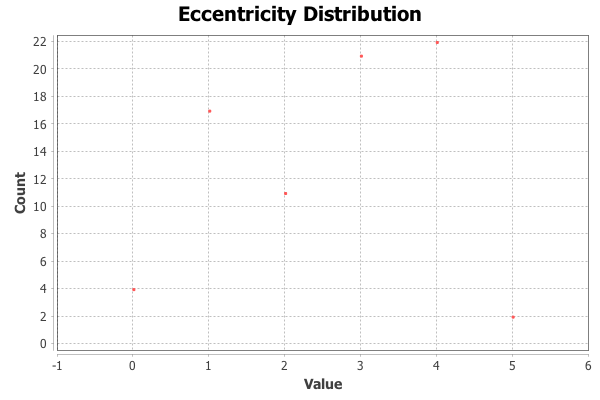
\includegraphics[width=12cm]{../images/eccentricity-distribution}
	\caption{Distribución de excentricidad para la red filtrada}
	\label{fig:eccentricity-distribution}
\end{figure}

En este gráfico (Figura \ref{fig:eccentricity-distribution}) vemos que hay bastantes nodos con distancia 0, esto es porque en el grafo hay nodos con grado de salida 0 y al ser una red dirigida es imposible llegar a ellos.
\\ \\
Recordamos, el diámetro de la red era 5 y la distancia media 2,4. En la distribución vemos como a mayor sea el valor de distancia, menor es el número de nodos. Esto es consecuencia de cumplir la propiedad de mundo pequeño. 

\subsection{Distribución de coeficientes de clustering}

El coeficiente de clustering de la red social es bastante bajo.
\\ \\

\section{Medidas de centralidad para nodos principales}
\label{sec:hubs}

En esta sección se va a intentar detectar a los actores principales dentro de la red según el grado.
\\ \\
Se presentarán en tablas con los 10 primeros actores y el valor que tienen para cada medida.

\begin{table}[H]
	\centering
	\caption{Actores principales según el grado}
	\label{tab:actores-principales-grado}
	\begin{tabular}{| l | l l l |}
		\hline
		\# & \textit{degree}       & \textit{in-degree}     & \textit{out-degree}   \\
		\hline
1  & [36] Valjean     & [32] Valjean        & [10] Marius         \\
1  & [22] Gavroche    & [18] Gavroche       & [10] Bossuet        \\
1  & [19] Marius      & [13] Thenardier     & [10] Joly           \\
1  & [17] Javert      & [12] Javert         &  [9] Fantine        \\
1  & [16] Thenardier  & [10] Enjolras       &  [9] Grantaire      \\
1  & [15] Enjolras    & [10] Myriel         &  [8] Courfeyrac     \\
1  & [15] Fantine     &  [9] Marius         &  [8] Bahorel        \\
1  & [13] Bossuet     &  [9] Eponine        &  [8] Claquesous     \\
1  & [13] Courfeyrac  &  [9] MmeThenardier  &  [8] Montparnasse   \\
1  & [12] Joly        &  [9] Tholomyes      &  [7] Babet          \\
		\hline
	\end{tabular}
\end{table}

\section{Comunidades}

Se ha utilizado Gephi para detectar comunidades dando una resolución de 1,5 y obteniendo 5 comunidades y un coeficiente de 0,545, el cual supera la barrera de 0,3 para considerarlo aceptable.
\\ \\

\begin{figure}[H]
	\centering
	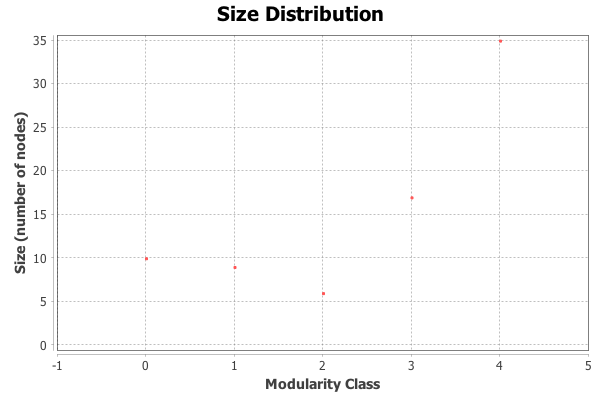
\includegraphics[width=12cm]{../images/communities-size-distribution}
	\caption{Distribución de comunidades en la red filtrada}
	\label{fig:communities-size-distribution}
\end{figure}

\begin{figure}[H]
	\centering
	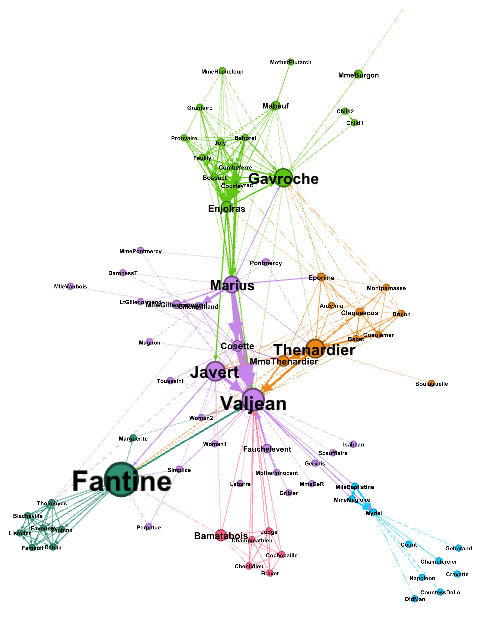
\includegraphics[width=12cm]{../images/modularity-class}
	\caption{Grafo de comunidades en la red}
	\label{fig:modularity-class}
\end{figure}






